% sample.tex
\documentclass{beamer}

\usetheme{boxes}

\usecolortheme[RGB={34,170,34}]{structure} 
\usepackage{amsmath}
\usepackage{amssymb}
\usepackage{graphics}
\usepackage{multicol}
\usepackage{color}
\usepackage[absolute,overlay]{textpos}
\usepackage{fancybox}

\usepackage{framed,color}
\definecolor{shadecolor}{rgb}{255,127,0}
\setbeamertemplate{itemize item}[circle]

\definecolor{verde}{RGB}{34,170,34}


\setbeamercolor{uppercolgreen}{fg=white,bg=verde!90}
\setbeamercolor{lowercolgreen}{fg=black,bg=verde!20}


%%%%%%%%%%%%%%%%%%%%%%%%%%%%%%%%%%%


\title[Shell Lesson]{Programming with Python}

\subtitle[]{EOAS Software Carpentry Workshop }
%\author[K. Ramos-Musalem ]{Karina Ramos Musalem}
\date[Sep 2015]{September 24nd, 2015}


%------------------ the document starts here -------------------------%

\begin{document}
\bibliographystyle{plainnat}
\bibliography{bib/biblio}


%------------------ the titlepage frame-------- -------------------------%

 
\begin{frame}[plain]
  
\titlepage


\end{frame}


%---------------- the presentation begins here --------------------%

%-------------------------- Intro ------------------------------------------%

\begin{frame}{Getting started}

\small{For our Python introduction we're going to pretend to be a researcher named Harold Bridge (user id \texttt{hbridge}) who is studying inflammation in patients who have been given a new treatment for arthritis.}
\vspace{0.5cm}

You need to download some files to follow this lesson:
\begin{enumerate}
 \item{Make a new folder in your Desktop called \texttt{python-novice-inflammation}.}
    \item{Download python-novice-inflammation-data.zip and move the file to this folder.}
    \item{If it's not unzipped yet, double-click on it to unzip it. You should end up with a new folder called data.}
   \item{You can access this folder from the Unix shell with:}
\end{enumerate}
\texttt{\$ cd \&\& cd Desktop/python-novice-inflammation/data}




\end{frame}

%-------------------------- jupyter notebook ------------------------------------------%

\begin{frame}{Launching Ipython (Jupyter) Notebook}

\small{There are several ways that we can use Python.  We're going to start with
a tool called Python Notebook that runs in the browser.
In a shell window enter these commands:}

\vspace{0.5cm}

\begin{beamerboxesrounded}[upper=uppercolgreen,lower=lowercolgreen,shadow=false]{}
\texttt{\$ cd \\
\$ cd Desktop/python-novice-inflammation/data \\
\$ ipython notebook}
\end{beamerboxesrounded}
\vspace{0.5cm}

\small{The shell window is now running a local web server for you.  Don't close it. You will need to open another shell window to do other command line things. Your browser should open to an "Jupyter:  Notebook" page showing a list of directories.}
\end{frame}

%-------------------------- AXIS ------------------------------------------%

\begin{frame}{Analyzing patient data}

\begin{enumerate}
    \item{Explain what a library is, and what libraries are used for.}
    \item{Load a Python library and use the things it contains.}
    \item{Read tabular data from a file into a program.}
    \item{Assign values to variables.}
    \item{Select individual values and subsections from data.}
    \item{Perform operations on arrays of data.}
    \item{Display simple graphs.}
\end{enumerate}
\end{frame}

%-------------------------- Challenge 01 ------------------------------------------%

\begin{frame}{ }
What does the following program print out?
\vspace{0.5cm}

\begin{beamerboxesrounded}[upper=uppercolgreen,lower=lowercolgreen,shadow=false]{}

\texttt{first, second = Grace' , `Hopper'}

\texttt{third, fourth = second, first}

\texttt{print (third, fourth)}

\end{beamerboxesrounded}

\end{frame}

%-------------------------- Challenge 01 - Solution ------------------------------------------%

\begin{frame}{ }
What does the following program print out?
\vspace{0.5cm}

\begin{beamerboxesrounded}[upper=uppercolgreen,lower=lowercolgreen,shadow=false]{}

\texttt{first, second = `Grace' , `Hopper'}

\texttt{third, fourth = second, first}

\texttt{print (third, fourth)}

\end{beamerboxesrounded}

\alert{ANSWER:}

\texttt{Hopper, Grace}
\end{frame}


%-------------------------- Challenge 02 ------------------------------------------%

\begin{frame}{ }
A subsection of an array is called a slice. We can take slices of character strings as well:

\begin{beamerboxesrounded}[upper=uppercolgreen,lower=lowercolgreen,shadow=false]{}

\texttt{element = `oxygen'\\
print `first three characters:', element[0:3]\\
print `last three characters:', element[3:6]\\}
\end{beamerboxesrounded}

\begin{enumerate}
\item{What is the value of element[:4]? What about element[4:]? Or element[:]?}
\item{What is element[-1]? What is element[-2]? Given those answers, explain what element[1:-1] does.}
 \item{The expression element[3:3] produces an empty string, i.e., a string that contains no characters. If data holds our array of patient data, what does data[3:3, 4:4] produce? What about data[3:3, :]?}
\end{enumerate}

\end{frame}

%-------------------------- AXIS ------------------------------------------%

\begin{frame}{Operations across an axis}

\begin{figure}[htbp]
   \centering
  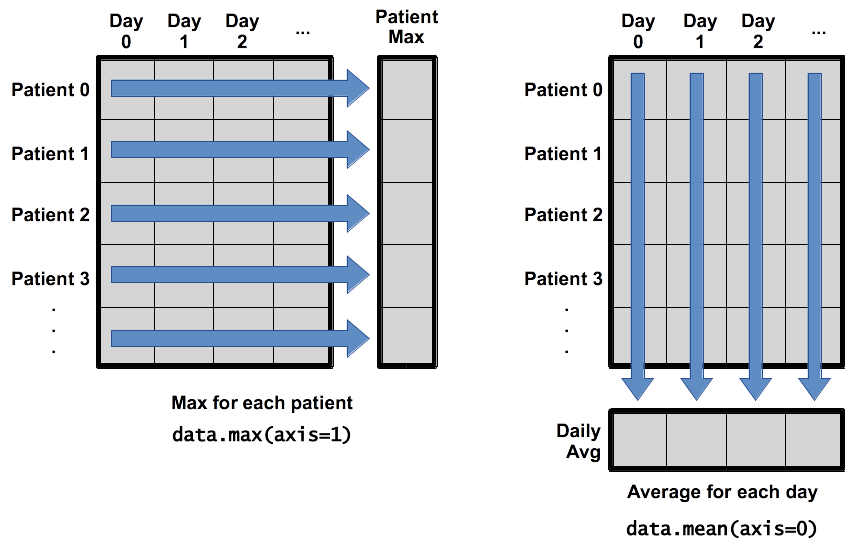
\includegraphics[width=0.7\textwidth]{figs_slides/python-operations-across-axes.png} 
\end{figure}

\end{frame}


%%-------------------------- Challenge 03 ------------------------------------------%

\begin{frame}{ }

\begin{enumerate}
   \item{ Why do all of our plots stop just short of the upper end of our graph? Why are the vertical lines in our plot of the minimum inflammation per day not vertical?}

   \item{ Create a plot showing the standard deviation of the inflammation data for each day across all patients.}
\end{enumerate}

\end{frame}

%%-------------------------- Challenge 04 ------------------------------------------%

\begin{frame}{ }

Modify the program to display the three plots on top of one another instead of side by side.

\end{frame}

%-------------------------- Challenge 05 - loops ------------------------------------------%

\begin{frame}{ }

Python has a built-in function called range that creates a list of numbers: range(3) produces [0, 1, 2], range(2, 5) produces [2, 3, 4], and range(2, 10, 3) produces [2, 5, 8]. Using range, write a loop that prints the first three natural numbers:

\vspace{0.5cm}

\begin{beamerboxesrounded}[upper=uppercolgreen,lower=lowercolgreen,shadow=false]{}
\texttt{1\\
2\\
3}
\end{beamerboxesrounded}

\end{frame}

%-------------------------- Challenge 05 - loops - My Sol------------------------------------------%

\begin{frame}{ }

Python has a built-in function called range that creates a list of numbers: range(3) produces [0, 1, 2], range(2, 5) produces [2, 3, 4], and range(2, 10, 3) produces [2, 5, 8]. Using range, write a loop that prints the first three natural numbers:

\vspace{0.5cm}

\alert{One solution:}

\texttt{for num in range(1,4,1):}

\texttt{      print(num)}
    

\end{frame}


%-------------------------- Challenge 06 - loops ------------------------------------------%

\begin{frame}{ }

Exponentiation is built into Python:

\vspace{0.5cm}

\begin{beamerboxesrounded}[upper=uppercolgreen,lower=lowercolgreen,shadow=false]{}

\texttt{print 5**3\\
125}
\end{beamerboxesrounded}

\vspace{0.5cm}

Write a loop that calculates the same result using multiplication (without exponentiation).
\end{frame}

%%-------------------------- Challenge 06 - loops - My Solution ------------------------------------------%

\begin{frame}{ }

Exponentiation is built into Python:

\vspace{0.5cm}

\begin{beamerboxesrounded}[upper=uppercolgreen,lower=lowercolgreen,shadow=false]{}

\texttt{print 5**3\\
125}
\end{beamerboxesrounded}

\vspace{0.5cm}

Write a loop that calculates the same result using multiplication (without exponentiation)

\alert{One possible answer:}

\texttt{ans=1}\\
\texttt{for ii in range(1,4,1):}\\
\texttt{      ans=ans*5}\\
\texttt{print(ans)}

\end{frame}

%-------------------------- the document ends here ----------------------------------%

\end{document}
